\section{Terminal mechanics}
\label{section:tty}
\epigraph{The tty layer is one of the very few pieces of kernel code that scares the hell out of me.}{Ingo Molnar\cite{molnarhell}}
You won't often need to deal with the gritty details of terminal access and
manipulation. It's still important to understand what's going on behind the
abstraction, especially for when things go wrong. As was made clear in
Chapters~\ref{sec:direct} and~\ref{sec:fullscreen}, Notcurses requires a
proper terminal definition and a handle to a terminal device, or initialization
will fail (NCURSES requires the same). With that said, the UNIX terminal layers
have never been, and are not now for the faint of heart\footnote{When Ingo
Molnar is scared, we all ought be scared.}. Extending back to the AT\&T dark
ages, they are configured primarily through messy \texttt{ioctl}s and the
slightly-less-messy \texttt{termios} API.

More details than you probably want are available from Chapters 18 and 19 of \cite{apiue}
(general UNIX), Chapters 62 and 64 of~\cite{linuxprogramming} and Chapter 18
of~\cite{linuxdevicedrivers} (Linux), and Chapter 10 of~\cite{freebsddesign} (FreeBSD).

Modern workstations support a variety of physical and virtual terminal devices:
\begin{denseitemize}
\item{Honest-to-Bog serial terminals, probably using the RS-232\cite{rs232}
      protocol over a D-subminiature 25-pin (DB-25M) or 9-pin (DE-9M)
      connector (see Table~\ref{table:serial}).}
\item{Virtual consoles on text-based video, plus a keyboard.}
\item{Virtual framebuffer consoles on graphics-based video, plus a keyboard.} 
\item{Terminal emulators in a graphical environment, plus brokered input devices.}
\item{Pseudoterminals hooked up to network connections.}
\end{denseitemize}

\begin{table}[!htbp]
  \centering
  \begin{tabular}{ |c|c|c|c|c| }
    \hline
    Signal & DB-25M & TIA-574 DE-9M & Yost 8P8C\cite{yost} & Originator \\
    \hline
    \hline
    Protective ground & 1 & x & x & x \\
    \hline
    Transmitted data & 2 & 3 & 3 & DTE \\
    \hline
    Received data & 3 & 2 & 6 & DCE \\
    \hline
    Request to send & 4 & 7 & 1 & DTE \\
    \hline
    Clear to send & 5 & 8 & 8 & DCE \\
    \hline
    Data set ready & 6 & 6 & 2 & DCE \\
    \hline
    Signal ground & 7 & 5 & 4, 5 & x \\
    \hline
    Carrier detect & 8 & 1 & 2 & DCE \\
    \hline
    Data terminal ready & 20 & 4 & 7 & DTE \\
    \hline
    Ring indicator & 22 & 9 & x & DCE \\
    \hline
  \end{tabular}
  \caption[RS-232/EIA-232 pin mappings]{RS-232/EIA-232 D-subminiature pins (DCE=Data circuit equip., DTE=Data terminal equip.)}
  \label{table:serial}
\end{table}

On Linux, three kernel definitions form the core of the terminal abstraction
(the ``tty layer''). A \texttt{tty\_driver} function interface exists for each
tty implementation, and each has a different corresponding
major+minor device number pair. These implementations are enumerated in
\texttt{/proc/tty/drivers} (sample contents are listed in Table~\ref{table:procttydrivers}).
Line disciplines can be found in \texttt{/proc/tty/ldiscs}. The only line discipline
you're likely to encounter in a terminal context is \texttt{n\_tty}, the ``new tty''
discipline responsible for implementing ``cooked mode''\cite{essentialdrivers}.

POSIX.1-2017\cite{posix2017} §10.1 ``Directory Structure and Devices''
specifies three special files in the \texttt{/dev} directory, of which two are
related to the terminal/console system: \texttt{/dev/tty} is, within a process
context, a synonym for the controlling terminal associated with that process's
group (this can also be acquired with \texttt{tty(1)} or the POSIX C function
\texttt{ctermid(3)}\footnote{\texttt{/dev/tty} also uniquely supports the
\texttt{TIOCNOTTY} \texttt{ioctl(2)} for detaching a process from its
controlling terminal.}. The tty associated with an arbitrary file descriptor can
be retrieved with \texttt{ttyname\_r(3)}). \texttt{/dev/console} is a generic name for the current system console\footnote{Defined in \textit{ibid.} §3.392
``System Console'' as the device receiving messages sent by the \texttt{syslog()}
function. On Linux, it will also reproduce messages written to \texttt{/dev/kmsg}\cite{dmesg}.};
POSIX requires that the system console implement its ``General Terminal Interface'' (see
\textit{ibid.} §11). \texttt{/dev/tty0} is a special device on Linux linked to
the current virtual console (which might not be the system console). The
available system consoles can be found in \texttt{/proc/consoles}.

Initial \texttt{/dev/ttyN} devices are created internally by the kernel
(according to the value of \texttt{MAX\_NR\_CONSOLES}, by default 64) and set
up by \texttt{udev}. These are distinct devices, each usable by one virtual
console. Serial consoles show up as \texttt{/dev/ttySN}\cite{ttys4}. Each
virtual console gets a device at \texttt{/dev/vcsN} allowing access to the
glyph values of the console, a device at \texttt{/dev/vcsaN} allowing access to
the attributes at each cell, plus screen geometry, and a device at \texttt{/dev/vcsuN}
providing access to the Unicode values of each cell. If a framebuffer console
is being used, these devices are prepared atop some framebuffer device \texttt{/dev/fbN} (see
Figure~\ref{fig:framebuffers}); these mappings can be managed with \texttt{con2fbmap(1)}.

\begin{figure}[!htbp]
  \centering
  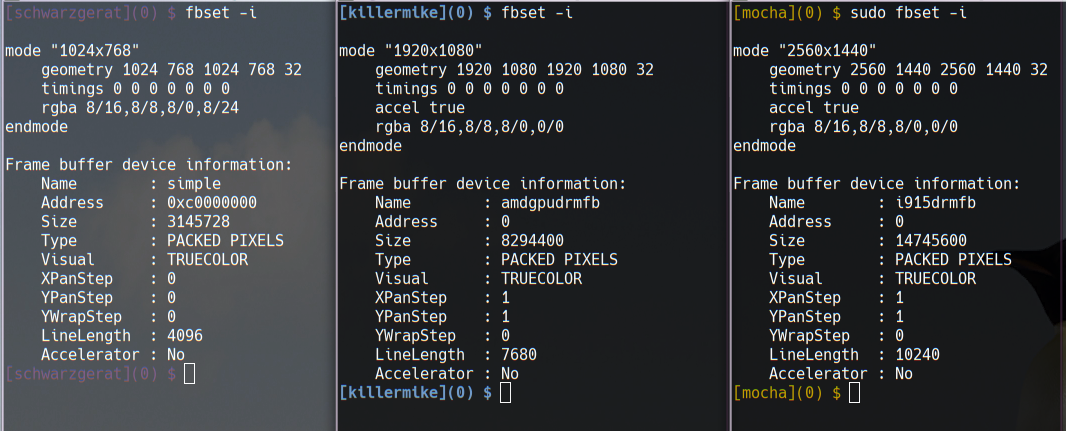
\includegraphics[width=.75\linewidth]{media/framebuffers.png}
  \caption{Three different Linux framebuffer implementations.}
  \label{fig:framebuffers}
\end{figure}

\begin{table}[!htbp]
  \centering
  \begin{tabular}{ |c|c|c|c|c|c| }
    \hline
    Name & Default node & Major & Minor & Type & sysfs \\
    \hline
    \hline
    /dev/tty & /dev/tty & 5 & 0 & system:/dev/tty & devices/virtual/tty/tty* \\
    \hline
    /dev/console & /dev/console & 5 & 1 & system:console & devices/virtual/tty/console \\
    \hline
    /dev/ptmx & /dev/ptmx & 5 & 2 & system & devices/virtual/tty/ptmx \\
    \hline
    /dev/vc/0 & /dev/vc/0 & 4 & 0 & system:vtmaster & x \\
    \hline
    usbserial & /dev/ttyUSB & 188 & 0--511 & serial & x \\
    \hline
    serial & /dev/ttyS & 4 & 64--95 & serial & x \\
    \hline
    rfcomm & /dev/rfcomm & 216 & 0--255 & serial & x \\
    \hline
    pty\_slave & /dev/pts & 136 & 0--1048575 & pty:slave & x \\
    \hline
    pty\_master & /dev/ptm & 128 & 0--1048575 & pty:master & x \\
    \hline
    unknown & /dev/tty & 4 & 1--63 & console & devices/virtual/tty/console \\
    \hline
  \end{tabular}
  \caption[Expanded contents of \texttt{/proc/tty/drivers}]{Extended content of a sample \texttt{/proc/tty/drivers}\\
    (5.5.6 kernel. \texttt{sysfs} information has been added)}
  \label{table:procttydrivers}
\end{table}

The various termios flags allow very fine control of the kernel state associated
with a given terminal. It is possible to mix flag settings arbitrarily, but three
modes are common, and have their own nomenclature:
\begin{denseitemize}
\item{\textbf{Canonical mode, aka cooked mode:}   The terminal driver buffers input until a newline is entered, while echoing
    it to the screen. Ctrl+C is mapped to \texttt{SIGINT}, Ctrl+\textbackslash\ is
    mapped to \texttt{SIGQUIT}, and Ctrl+Z is mapped to \texttt{SIGTSTP}.
    Buffered input is flushed when these signals are sent. The default mode
  under SUS4.}
\item{\textbf{Cbreak mode:} Line buffering is disabled, as is the processing
  of erase/kill characters. Interrupt and flow control translation is unaffected.
Sometimes referred to as \textit{rare mode}. This mode allows processing of input
without waiting for a newline character, while retaining e.g. Ctrl+C.}
\item{\textbf{Raw mode:} Interrupt and flow control translation is also disabled.
  This allows all keyboard input to be processed without preprocessing by the
  line discipline, but e.g. Ctrl+C behavior is lost, and (if desired) must be
  emulated in user space.}
\end{denseitemize}

In addition to these physically-backed devices, ptys---pseudoterminal devices\cite{pty7}---exist
to support virtual teletype functionality, wherein a process plays the role
of hardware. Pseudoterminals\footnote{You might
 hear about both System V and BSD pseudoterminals. SUS standardized around
the System V form, known on Linux as ``UNIX 98''. This term refers to 1997's
SUSv2. BSD ptys look like \texttt{/dev/ttyLN} and \texttt{/dev/ptyLN}, and are
garbage.} back most terminal instances, including GUI terminal emulators, network
services such as SSH, and multiplexers such as \texttt{screen}. A pty provides a
bidirectional channel between a \textit{master} and \textit{slave}, with the
slave presenting a classic terminal interface (i.e. writing a Ctrl+C to the
master side will (under the cooked or cbreak disciplines) result in
\texttt{SIGINT} being delivered to the foreground process group.

The details of Linux pseudoterminal pair creation can be found on the \texttt{pts(4)}\cite{pts4} man page.
%\texttt{posix\_openpt(3)}\cite{posixopenpt3} opens the ``master clone device''
%\texttt{/dev/ptmx}, receiving a file descriptor corresponding to the new PTM
(pseudoterminal master).
A new PTS (pseudoterminal slave) is created in
%\texttt{/dev/pts/}
%\footnote{\texttt{/dev/pts} is typically its own \texttt{devpts} filesystem on Linux.}
, whose name can be discovered by
%providing the PTM file descriptor to \texttt{ptsname\_r(3)}\cite{ptsname3}.
Opening this PTS requires use of the \texttt{grantpt(3)} and \texttt{unlockpt(3)} calls.
Once both sides have been opened, data freely flows between the PTM and PTS.

You generally shouldn't need to be mess with TTYs or PTYs yourself as an
application developer, but it's important to know what's going on\footnote{Pro
tip: should you ever need supply input to programs which refuse to read from
pipes (e.g. \texttt{passwd}), you can pump the input through a named pty.}.

\subsection{Terminals and the UNIX process model}
\label{sec:unixprocs}

Understanding how these devices

You're hopefully aware that UNIX programs traditionally start with at least
three file descriptors open: 0 for \texttt{stdin}, 1 for \texttt{stdout}, and 2
for \texttt{stderr}. 
\textbf{FIXME FIXME acquisition of a tty (getty->login, ssh->pty),
  internals of kernel tty/pty devices, session groups, signal distribution,
  \texttt{/dev/tty} and \texttt{/dev/ttyXX}s}
My diagrams are adapted in part from those of Linus Akesson\cite{ttydemystified}.
\textbf{FIXME diagrams!}

\textbf{cover systemd-logind, getty, logind.conf, sd-login}
\subsection{Escape codes ANSI and otherwise}
\label{sec:escapes}

In a relic from teletypes, ISO 646, ISO 2022, and ECMA-35 described use of
non-destructive backspace to produce composed characters from spacing ones.
This had been eliminated by ISO 4873, ECMA-43, and ISO 8859.

\textbf{FIXME FIXME other stuff}
